\chapter{Secure web browsers with virtualisation}\label{bubble}

\epigraph{2in}{Computers are useless. They can only give you answers.}{Pablo Picasso}{}


Although virtualisation technology appeared to fulfil the needs of server consolidation and to optimise energy consumption within data centers, another growing trend that has been observed into marketplace is known as \emph{virtual desktop}.
It seems that the tendency of centralising data has been extended to the desktop environment. Desktop virtualisation is taking advantage of hypervisor-based technology for delivering applications, data and entire desktop environments to users. 
Traditional countermeasures that have been designed for those applications that are now delivered on-demand do not benefit of the diverse execution context. 
We are confident that hypervisor-awareness can lead to stronger security measures, better user experience and, above all, minimal performance impact.

\section{Motivation}
One of the most considerable actors in today's computer use is the web browser. Companies like Google\texttrademark and Yahoo are evidence of this trend since they offer full-fledged software inside the browser. 
This has resulted in a very rich environment that is being used by web programmers too. Unfortunately, an immediate side effect of this tendency is the growth of security problems like cross site scripting and cross site request forgeries (CSRF) \cite{xss,csrf,csrf2}. 
Moreover, the browser is often written in unsafe languages. As in any other software of this type, the web browser is exposed to the various vulnerabilities that can affect programs written in such languages, such as buffer overflows, dangling pointer references, format string vulnerabilities, memory corruption, etc.
One of the most often exploited type of C/C++ vulnerability of the last decade has been the stack-based buffer overflow \cite{dalton2008real}. Countermeasures like StackGuard \cite{Wagle:2003:SGS}, ProPolice \cite{Etoh:2000:PSS} and other tools like those explained in \cite{dep, wilander2003comparison} that protect areas of potential interest for attackers from being modified, have made buffer overflows harder to exploit. 
As a consequence, in the constantly animated attacker-researcher world, attackers have focussed on other types of vulnerabilities, targeting the heap rather than the stack. 
This has massively increased the number of heap-based buffer overflows and memory corruption attacks.

However, due to the changing nature of the heap, these types of vulnerabilities are notoriously harder to exploit.
Specifically to the web browser, the heap can look completely different depending on which and how many web sites the user has been visiting. It will be hard for attackers to figure out where in the heap space an exploitable overflow has occurred in order to locate  and execute their injected code.
Countermeasures like ASLR (Address Space Layout Randomisation) \cite{Bhatkar:2003:AOE} specifically designed to protect the heap have made it even harder to reliably exploit these types of vulnerabilities. In fact, ASLR is a technique by which positions of key data areas in a process's address space, such as the heap, the stack or libraries, are re-arranged at random locations in memory. 
All attacks based on the knowledge of target addresses (e.g. \emph{return-to-libc} attacks in the case of randomised libraries or attacks that execute injected \emph{shellcode} in the case of a randomised heap/stack) may fail if the attacker cannot guess the exact target address.

Recently a new attack emerged that combines the richer environment found in the browser to facilitate exploits of vulnerabilities based on unsafe languages, sometimes even resulting in the successful bypass of countermeasures like ASLR, which are supposed to protect against these types of vulnerabilities.
One such attack is known as \textit{heap-spraying}. The name depicts its nature of using the Javascript engine, usually embedded within modern web browsers, to replicate the code that attackers want executed, a large number of times inside the heap memory. As a result, the chances that a particular memory location in the heap will contain their code will dramatically increase. 

Back in 2009 a cyber attack called Operation Aurora \cite{aurora} targeted several organisations such as Google, Adobe, Yahoo, Symantec, Morgan Stanley and others, with the sole purpose of stealing intellectual property. The attack achieved many of its goals by a coordinated set of operations that included the execution of malicious Javascript which included a zero-day exploit within the Internet Explorer web browser. The exploit downloaded a binary, executed its payload to set up a backdoor and connected to command and control servers.
After such attack was publicly disclosed, code snippets with similar behaviour affected a series of applications that, equally to the web browser, are equipped with script environments and are thus vulnerable to the same type of attack \cite{iespray,safarispray,ffspray}.

In the first part of this chapter we focus on modern web browsers and describe a countermeasure against a memory corruption attack such as heap-spraying. In the second part we discuss how the aforementioned countermeasure can be integrated and benefit of the virtualisation-based environment that delivers the protected application on-demand.

The rest of the chapter is organised as follows: Section \ref{bub:problem} discusses the problem of heap-based buffer overflows and heap-spraying in more detail. Section \ref{bub:approach} discusses our approach while in Section \ref{bub:implementation} we describe our prototype implementation. We evaluate our approach in Section \ref{bub:eval}. 
A discussion about the integration within hypervisor-aware systems is given in Section \ref{bub:integration}. We compare our approach to related work in Section \ref{bub:related}. Section \ref{bub:conclusion} concludes.

\section{Problem description} \label{bub:problem}
\paragraph{Heap-based buffer overflows}
The first step to deploy a heap-spraying attack successfully consists in the injection of malicious code at an arbitrary memory location. 
Designing security countermeasures assumes that an exploitable vulnerability might exist. This is considered the minimal condition for an attacker to change the execution flow of the program and jump to the injected code.
%Once this location has been traced, the attacker can jump to that code in order and trigger the attack. 
Because a memory corruption is required, heap-spraying attacks are considered a special case of heap-based attacks. 
Exploitable vulnerabilities for such attacks normally deal with dynamically allocated memory. 
A general way of exploiting a heap-based buffer overflow is to overwrite management information that the memory allocator stores next to the actual data. General purpose memory allocators, as the ones present in commodity operating systems, allocate memory in chunks. These chunks are usually located in a doubly linked list and contain both memory management information (referred to as \textit{chunkinfo}) and real data (referred to as \textit{chunkdata}). Several allocators have been attacked by overwriting the \textit{chunkinfo} section \cite{younan2005security}. 

%TODO fig heapover and description
%Fig. \ref{heapover} shows a heap-based buffer overflow attack on the Linux memory allocator by overflowing a buffer located in \emph{chunk1}. Memory management information is overwritten and modified to the attacker's desire.

%The forward pointer (\textit{fd}) is changed to point twelve bytes before function \texttt{f0}'s return address, while the backward pointer (\textit{bk}) is changed to point to code that will jump over the next few bytes and execute the injected code. When \emph{chunk1} is freed, it is coalesced with \emph{chunk3}. As \emph{chunk3} is no longer a separate chunk after the coalescing, it must first be removed from the list of free chunks (\textit{unlinking}). Internally a free chunk is represented by a data structure containing the fields depicted in \emph{chunk3} in Fig.\ref{heapover}. The unlinking of \emph{chunk3} occurs as follows:
%\\
%\emph{chunk3 $\rightarrow$ fd $\rightarrow$ bk  = chunk3 $\rightarrow$ bk\\
%chunk3 $\rightarrow$ bk $\rightarrow$ fd  = chunk3 $\rightarrow$ fd\\
%}
%\\
%When \emph{chunk3} is unlinked, the value of the memory location that is twelve bytes after the location pointed to by \emph{fd} will be overwritten with the value of \emph{bk}, and the value of the memory location eight bytes after the location pointed to by \emph{bk} will be overwritten with the value of \emph{fd}. As a result, the return address will be overwritten with a pointer to code that will jump over the place where \emph{fd} will be stored and the injected code will be executed. 
%%Once malicious code has been injected, the attack will complete successfully if it is executed. 
Since the heap memory area is much less predictable than the stack it would be difficult to predict the memory address to jump to and execute the injected code. Some countermeasures have contributed to making these vulnerabilities even harder to exploit \cite{Younan04codeinjection, Erlingsson:2007:LAD}. 

\paragraph{Heap-spraying attacks}
As mentioned before, an effective countermeasure against attacks based on heap-based buffer overflow is Address Space Layout Randomisation (ASLR) \cite{Bhatkar:2003:AOE}. ASLR is a technique which randomly arranges the positions of key areas in a process's address space. This would prevent the attacker from easily predicting target addresses. 
However, attackers have developed more effective strategies that can even bypass these countermeasures. 
Heap spraying \cite{heapspray} is a technique that will increase the probability to land on the desired memory address even if the target application is protected by ASLR. Heap spraying is performed by populating the heap with a large number of objects containing the attacker's injected code.
The act of spraying simplifies the attack and increases its likelihood of success.
This strategy has been widely used by attackers to compromise security of web browsers, making attacks to the heap more reliable than in the past while opening the door to bypassing countermeasures like ASLR \cite{ffspray,pdfspray,asspray,iespray,safarispray}.

A heap-spraying attack attempts to increase the probability to jump to the (\texttt{shellcode}). To achieve this, a basic block of NOP\footnote{Short for No Operation Performed, is an assembly language instruction that effectively does nothing at all \cite{32intel}} instructions is created. The size of this block is increased by appending the block's contents to itself, building the so called \textit{NOP sled}. Alternatively, a code semantically equivalent to \texttt{No Operation} might be used and have the same effect of increasing the size of the block. This technique can also circumvent trivial countermeasures that rely on simple NOP code detection.
Finally \texttt{shellcode} is appended to the block of instructions. Therefore a jump to any location within the \textit{NOP sled} will sooner or later transfer control to the \texttt{shellcode} appended at the end. 
Clearly, the bigger the sled (or, equally, the higher the number of sleds) the higher the probability to land in it (or to land in one of them) and the attack to succeed.

A schema of the object described above is provided in Fig.\ref{NOPfig}. 

\begin{figure}[htbp] 
\begin{center}
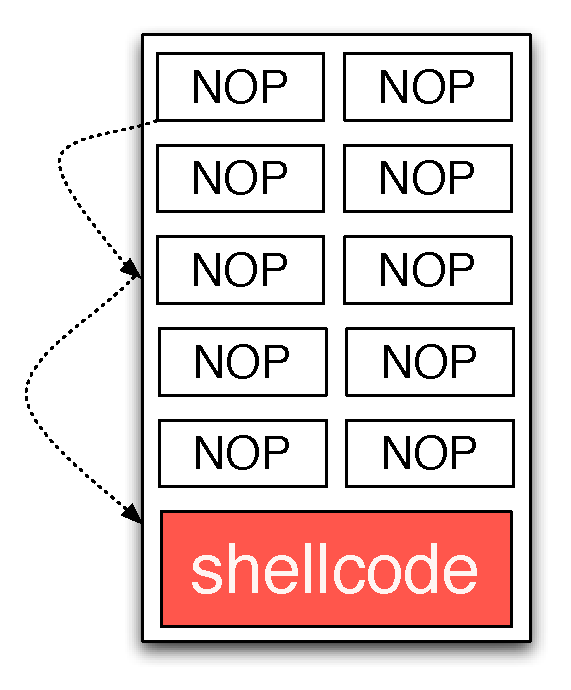
\includegraphics[scale=0.35]{images/nop_shellcode}
\caption{{Schema of NOP sled and shellcode appended to the sequence}}
\label{NOPfig}
\end{center}
\end{figure}

The second phase of the attack consists in populating the heap by exploiting the legal constructs provided by the scripting language embedded in the browser. Figure \ref{heapattack} shows the schema of a heap-spraying attack while populating the  heap.

 \begin{figure*}[htbp]
 \begin{center}
 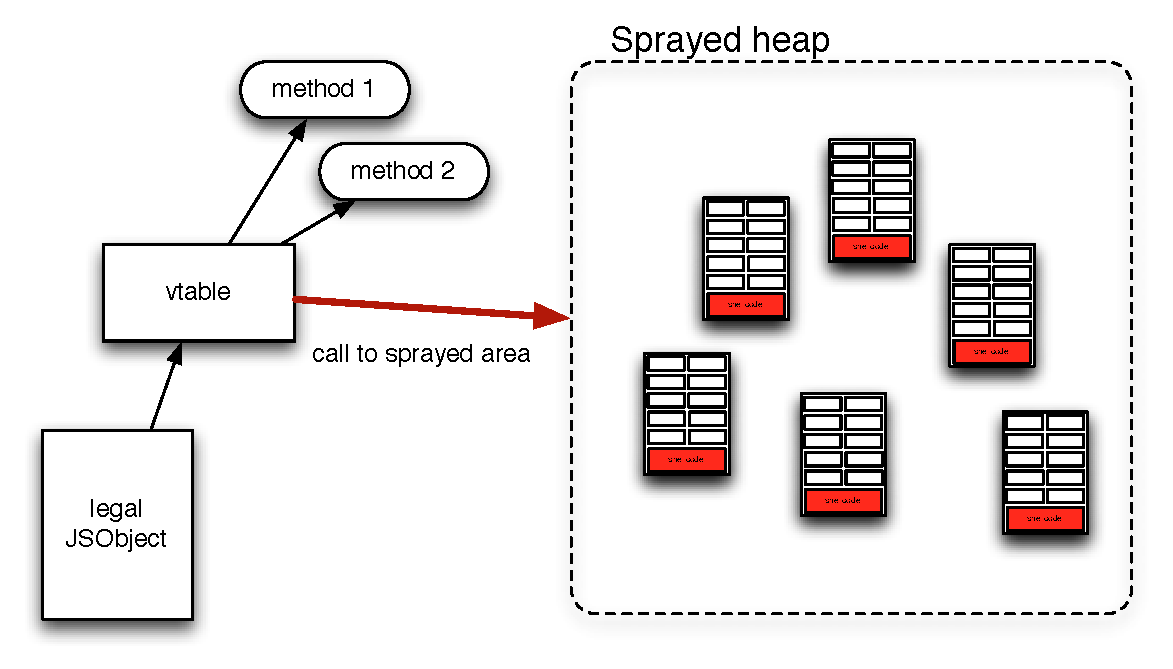
\includegraphics[scale=0.5]{images/attack}
 \caption{{A heap-spraying attack: heap is populated of a large number of $NOP-shellcode$ objects. The attack may be triggered by a memory corruption. This could potentially allow the attacker to jump to an arbitrary address in memory. The attack relies on the chance that the jump will land inside one of the malicious objects.}}
 \label{heapattack}
 \end{center}
 \end{figure*}

Although we will refer to spraying the heap of a web browser, this exploit can be used to spray the heap of any process that leaves to the user the ability to allocate objects into memory. For instance a popular PDF viewer has been found vulnerable to heap-spraying attacks. In that case, a forged PDF file was the medium to execute arbitrary code \cite{adobereader}.

What makes heap-spraying an unusual security exploit is the fact that the action of spraying the heap is considered legal and should be permitted by the application. In our specific scenario, memory allocation may be the regular behaviour of the browser while surfing benign web pages. Modern web sites that use AJAX (Asynchronous Javascript And XML) technology or plain Javascript (i.e. facebook.com, economist.com, ebay.com, yahoo.com and many others) appear as they are spraying the heap since a large number of objects is usually downloaded and allocated during their normal operation. 
We are aware that a security countermeasure should not prevent an application from allocating memory. This makes heap-spraying detection a challenging problem to deal with.


\begin{lstlisting} [label=some-code,caption=A Javascript code snippet to perform a basic heap-spraying attack usually embedded in a HTML web page]

 1. var sled;
 2. var spraycnt = new Array();
 3. sled = <NOP_instruction>; 
 4. while(sled.length < _size_)  
 5.   {
 6.     sled+=sled;
 7.   }
 8. for(i=0; i< __very_large__; i++)
 9.   {
 10.   spraycnt[i] = sled+shellcode;		
 11. }
\end{lstlisting}
 \label{snippet}

Because the layout of the heap depends on how often the application has allocated and freed memory, triggering an attack without any knowledge of the exact location to jump to, is utterly difficult. The attacker's strategy would be reduced to merely guessing the address where the malicious objects have been injected to.
Unfortunately, by using a client-side scripting language, such as Javascript, it is possible to arrange the heap to the desired layout, making the attack more reliable as described in \cite{heapfengshui, engheap}.

Code in Listing \ref{snippet} shows a basic heap-spraying attack in Javascript (without any attempt of arranging  the heap layout in order to better locate the injected code).

%%\subsection{JIT-spraying attacks}

\section{Approach}\label{bub:approach}
An important property of a heap-spraying attack is that it relies on homogeneity of memory. This means that it expects large parts of memory to contain the same information. It also relies on the fact that landing anywhere in the \texttt{nopsled} will cause the shellcode to be executed. 
The key of our countermeasure consists in introducing diversity on the heap, breaking the assumption of homogeneity and making it much harder to reach the shellcode and thus trigger the attack.
 
The first known heap-spraying attack used the Javascript string type to build sleds. We explain our approach accordingly. 
The assumption is broken by inserting special interrupting values at random positions whenever the string is stored into memory and removing them whenever the string is used by the application. If these special interrupting values are executed as an instruction, the program will generate an exception that will be served by an interrupt handler that has been previously installed.

Because these special values interrupt the strings inside the memory of the application, the attacker can no longer depend on the NOP sled or even the shellcode being intact. If these values were placed at fixed locations, the attacker could attempt to bypass the code by inserting jumps over specific possible locations within the code. Such an attack, however is unlikely, because the attacker does not know exactly where inside the shellcode control has been transferred.

To make the attack even harder, the special interrupting values are placed at random locations inside the string. Since an attacker does not know at which locations in the string the special interrupting values are stored, he can not jump over them in his NOP-shellcode. This lightweight approach thus makes heap-spraying attacks significantly harder at very low cost.
%%Surfing a malicious web site would be sufficient to expose a regular web browser to the risk of a heap-spraying attack.
%%As described in Section \ref{sec:problem} an object used to spray the heap may be formed by a sequence of NOP instructions and a  shellcode appended to it. A number of such objects are then allocated on the heap by using the constructs offered by the browser-supported language.
%%In the typical scenario a Javascript string will contain the NOP sled and the shellcode.
%%The snippet shows how a Javascript array may be filled up with a large amount of entries, each containing the NOP-shellcode string\footnote{A realistic attack might fill \texttt{sled} and \texttt{spraycnt} by an image or media. For our proof of concept we will use Javascript strings since with this simple approach it is not required the user to download anything: all objects can be built locally.} .\\
%%The NOP instructions will increase the likelihood that the attack will succeed. After triggering the attack, if the instruction pointer falls at any position within the NOP sequence, it will be transfered to the shellcode appended at the end. \\
%%Basically if the NOP sled is interrupted, by special values, at random positions, it would be harder to reach the shellcode from the sled. Also in the case where the NOP sled is a more complex sequence with \texttt{jump} instructions, introducing diversity would dramatically decrease the probability that the attack will be successful.
%%Since we cannot prevent the allocation of new memory, our approach would prevent the execution of the contents of malicious objects.\\
We have implemented this concept in the Javascript engine of Mozilla Firefox, an open source web browser.

The internal representation of Javascript strings has been modified in order to add the interrupting values to the contents when in memory and remove them properly whenever the string variable is used or when its value is read. The amount of interrupting values can be tuned via a parameter that is set at browser build time. The highest degree of security of our approach can be guaranteed by setting to $s=25$ bytes the maximum interval at which interrupting. The smallest useful shellcode found in the wild \cite{smallshell} at the time of writing would not fit in this interval. 
For less strict security requirements, larger values can be assigned to the parameter $s$.

Given the length $n$ of the string to transform $i=\lceil \frac{n}{25} \rceil$ intervals are generated (where $n>25$). A random value is selected for each interval. These numbers will represent the positions within the string to modify. The parameter sets the size of each interval, thus the number of positions that will be modified per string. Obviously by choosing a lower value for the parameter $s$ the amount of special interrupting values $i$ that are inserted will be increased and so will the overall performance impact.
However, setting the size of each interval to the length of the smallest shellcode does not guarantee that the positions will be at a distance of $25$ bytes. It may occur that a position $p$ is randomly selected from the beginning of its interval $i_{p}$ and the next position $q$ from the end of its interval $i_{q}$. In this case $(q-p)$ could be greater than $25$, allowing the smallest shellcode to be stored in between. 
Nevertheless what makes heap-spraying attacks reliable is the large amount of homogeneous data, not simply the insertion of shellcode. Thus being able to insert shellcode will not simply allow an attacker to bypass this approach.

When the string characters at random positions have been changed, a support data structure is filled with \textit{metadata} in order to keep track of the original values and their locations within the string. The modified string is then stored into memory. Whenever the string variable is used, the engine will perform an inverse function, to restore the original content of the string and return it to the caller. This task is achieved by reading the metadata from the data structure bound to the current Javascript string and replacing the special interrupting values with their original content on a copied version of the string. With this approach different strings can be randomised differently, giving the attacker even less chances to figure out the locations of the interruptions. 
%Because each string variable stays modified as long as it is stored in memory and a copy of this string variable is only restored to its original content when the application requests access to that a string. 
When the function processing the string stores the result back to memory, the new string is again processed by our countermeasure. If the function discards the string, it will simply be freed. Moreover the Javascript engine considered here implements strings as immutable type. This means that string operations do not modify the original value. Instead, a new string with the requested modification is returned.  


\section{Implementation}\label{bub:implementation}
In this section we discuss the implementation details of our countermeasure and the strategy we considered to tailor it on the Javascript engine of Mozilla Firefox web browser.
An attacker performing a heap-spraying attack attempts to arrange a contiguous block of values of his choice in memory. This is required to build a sled that would not be interrupted by other data. To achieve this, a monolithic data structure is required.
Javascript offers several possibilities to allocate blocks in memory. The types supported by the Javascript engine in our prototype are numbers, objects and strings. An overview about how the Javascript engine represents Javascript objects in memory is given in \cite{jsobj}. 

%%Most objects have a prototype (which is another object) to inherit methods from, a parent to implement lexical scoping and properties 
%%[FIXME: write something about how each of the object types are stored in memory and why they are not a threat!] 
The string type represents a threat and can be used to perform a potentially dangerous heap-spraying attack. Figure \ref{jsstring} depicts what a \texttt{JSString}, looks like.  It is a data structure composed of two members: the \texttt{length} member, an integer representing the length of the string and the \texttt{chars} member which points to a vector having byte size \texttt{(length + 1) * sizeof(jschar)}. When a string is created, \texttt{chars} will be filled with the real sequence of characters, representing that contiguous block of memory that the attacker can use as a sled. 

\begin{figure}[htbp]
\begin{center}
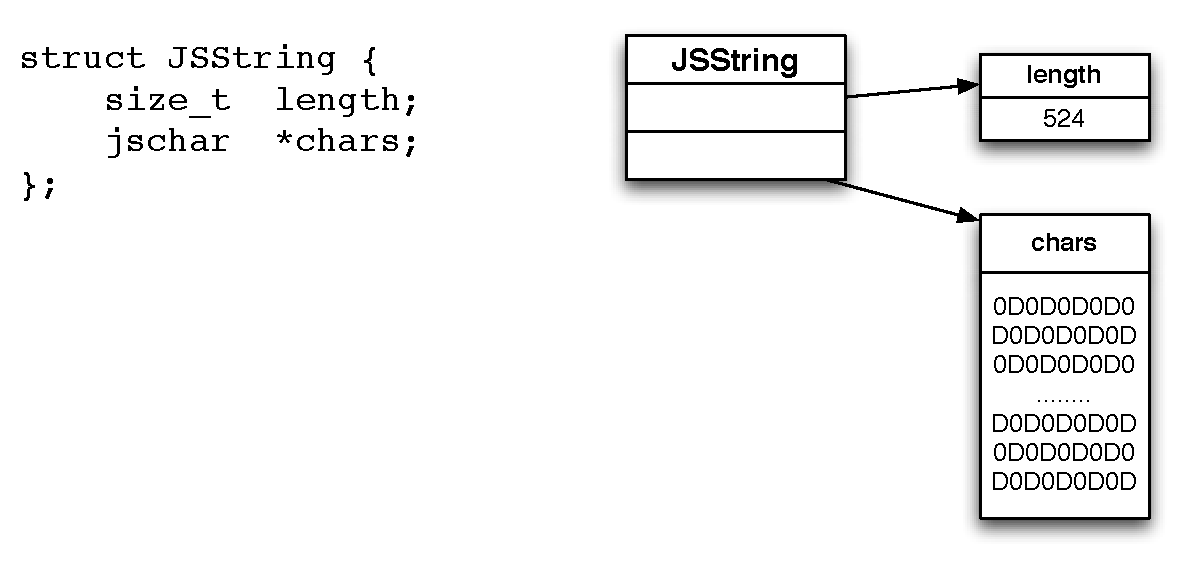
\includegraphics[scale=0.4]{images/jsstring.pdf}
\caption{{Javascript engine's JSString type is considered a threat for a heap-spraying attack since member \emph{chars} is a pointer to a vector of size ($length+1$)* \emph{sizeof(jschar)} }}
\label{jsstring}
\end{center}
\end{figure}

We have instrumented the \texttt{JSString} data structure with the fields to store the metadata: a flag $transformed$ will be set to $1$ if the character sequence has been transformed and an array $rndpos$ is used to store the random positions of the characters that have been modified within the sequence.

\begin{figure}[htbp]
\begin{center}
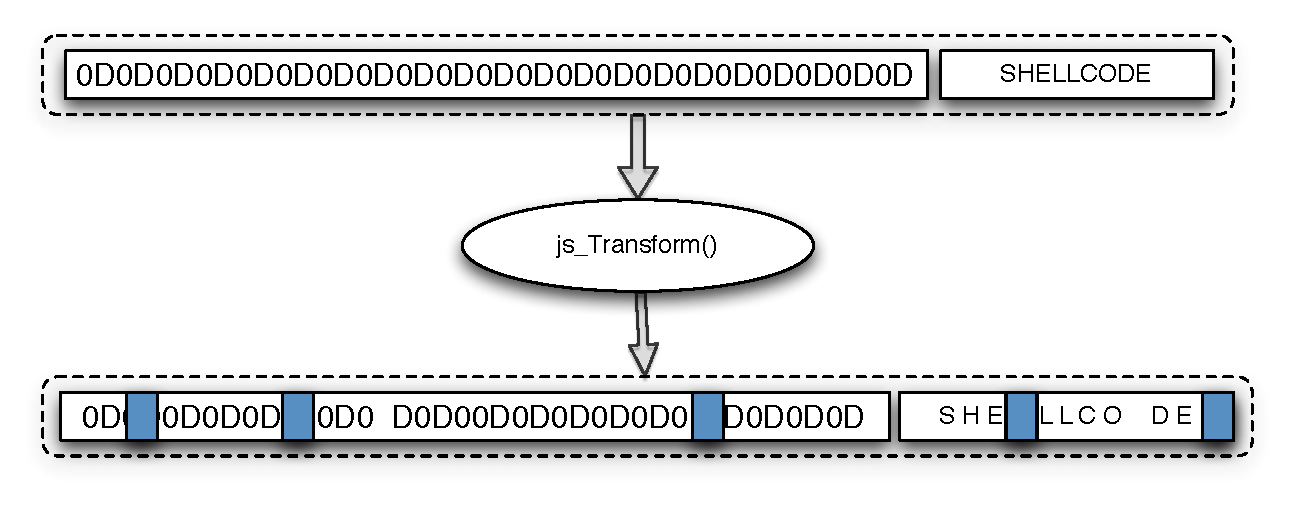
\includegraphics[scale=0.5]{images/stringint}
\caption{{Representation of the transformed string in memory: characters at random positions are changed to special interrupting values. The potential execution of the object's contents on the heap would be interrupted by the special value (in blue).}}
\label{stringrepr}
\end{center}
\end{figure}

Our countermeasure will save the original value of the modified character to $rndpos$, change its value (at this point the string can be stored into memory) and will restore the original value back from $rndpos$ whenever the string is read.

This task is performed respectively by two functions:\\
\texttt{js\_Transform(JSString*)} and \texttt{js\_Restore(JSString*)}.

The value of the character to modify is changed to the 1-byte value \texttt{0xCC}. This is the assembly language instruction for x86 processors to generating a software breakpoint. If a heap-spraying attack has been successfully triggered\footnote{The instruction pointer has been forwarded to an arbitrary location within one of the sprayed NOP-sleds} and the byte \texttt{0xCC} at a random position has been executed, an interrupt handler will detect and report the attack. This alert usually results in exposing a visible popup that encourages the user to close the application and notify the browser's vendor of the detected issue.

As mentioned in Section \ref{bub:approach}, the number of characters to randomise depends on the $s$ parameter. This parameter was chosen based on the length of the smallest shellcode found (to date, 25 bytes long\footnote{The smallest setuid and execve shellcode for GNU/Linux Intel x86 to date can be found at \url{http://www.shell-storm.org/shellcode/files/shellcode-43.php}}), but can be tuned to select the level of security and the overhead that will be introduced by the countermeasure.
If $size$ is the length of the string to transform, the number of intervals is given by $\lceil \frac{size}{24} \rceil $. 
A random value for each interval will represent the position of the character that will be changed. 
For reducing the impact of the countermeasure, $50$ random values in the range $(0,24)$ are generated at browser startup. These values are used as offsets to add to the first index of each interval to compute the random position within that interval. The random values are regenerated whenever the Garbage Collector reclaims memory. This prevents an attacker from learning the values over time as they may already have changed.

The value of the $i^{th}$ random position is stored at $rndpos[2i]$, while the original value of the $i^{th}$ character is stored at $rndpos[2i+1]$, with $i=0,1,2\dots$. Figure \ref{rndposarray} provides a schema of how these (position, character) pairs are stored.

Finally, function \texttt{js\_Transform(str)} will use the values stored in the \\
$str$ $\rightarrow$ $rndpos[]$ array to restore the string to its original content.
	
\begin{figure}[t]
\begin{center}
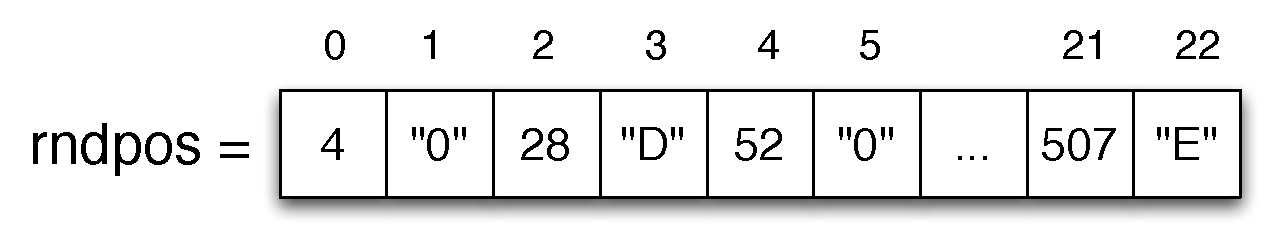
\includegraphics[scale=0.4]{images/rndpos}
\caption{{How metadata is stored to array $rndpos$: index $i$ within the array contains the value of the position in the string; index $(i+1)$ contains its original value}}
\label{rndposarray}
\end{center}
\end{figure}



\section{Evaluation} \label{bub:eval}
In this section we discuss the performance overhead measured by executing our proof-of-concept on a machine with  hardware specifications reported in Table \ref{machinespecs}. The reference environment consists of Mozilla Firefox (Ver. 3.7 Beta 3) browser \cite{mozilla} equipped with ECMA-262-3-compliant Javascript engine, Tracemonkey (Ver. 1.8.2)\cite{ECMA-262}.

We report results of macro benchmarks in order to assess the impact on user experience and micro benchmarks for  measuring the real overhead. An analytical study of the memory overhead in the worst case scenario is provided too. By \textit{worst case} we mean the case in which it is guaranteed that the smallest shellcode cannot be stored on the heap without being interrupted at least once by the \texttt{0xCC} byte.
Last but not least, we made a probabilistic analysis to evaluate the chances of an attacker who can execute shellcode without being detected.
%In Section \ref{perfover} we discuss our performance overhead, while in Section \ref{anal} we report an analytical study of the memory overhead in the worst case\footnote{With \textit{worst case} we mean the case where it is guaranteed that the smallest shellcode cannot be stored on the heap without being interrupted by random bytes.}.
%All benchmarks were performed on an Intel Core 2 Duo 2Ghz, 4GB RAM, running Debian Gnu/Linux. 

\subsection{Performance benchmarks} \label{perfover}
\paragraph{Macro-benchmarks}
To collect timings of the overhead in a real life scenario, a performance test similar to the one used in Nozzle \cite{nozzle08tr} has been used. Nozzle is the first countermeasure that has been specifically designed to mitigate heap-spraying attacks.
We downloaded and instrumented the HTML pages of eight popular web sites by adding the Javascript \texttt{newDate()} routine at the beginning and at the end of the page, and computed the difference between the two values. This number represents the time it takes to load the page and execute the Javascript code. Since the browser caches the contents of the web page, that value is a good approximation of the time needed for executing the Javascript.
We perform the benchmark 20 times for each website, 10 times with countermeasure disabled and 10 times with countermeasure in place. Table \ref{perfpopular} shows that the average performance impact over these websites is below 5\%.

\begin{table*}[htdp]
\begin{center}
\begin{tabular}{|c|c|c|c|} 
\hline
\bf{Site URL} & \bf{Load w/o [ms]} & \bf{Load w [ms]} & \bf{Perf. overh.} \\
\hline
economist.com 	& 	17304 	& 	18273	&  +5.6\% \\ 
amazon.com    	&      11866  	&  	12423 	&  +4.7\% \\
ebay.com 		&      7295  	&  	7601  	&+4.2\% \\
facebook.com 	&      8739  	&  	9167 	& +4.9\%\\ 
maps.google.com &  15098	&	15581       & +3.2\%\\
docs.google.com	& 426	&	453		& +6.3\%\\
cnn.com     	&      12873 	&  	13490 	&+4.8\%\\ 
youtube.com 	&      12953 	&  	13585    	& +4.9\%\\
\hline
\bf{Average}  &   &   & \bf{+4.82}\\ 
\hline
\end{tabular}
\end{center}
\vspace{-0.3cm}
\caption{{ Performance overhead of countermeasure in action on 8 popular memory demanding web sites.}}
\vspace{0.3cm}
\label{perfpopular}
\end{table*} 

We consider the aforementioned performance overhead small and the overall countermeasure fast enough for every day computing, due to the fact that the time for loading a web page is usually relatively short to have a noticeable impact on user experience.

\paragraph{Micro-benchmarks}
Micro-benchmarks can offer a better evaluation of the real performance impact. We performed three different benchmarks: the SunSpider Javascript Benchmarks \cite{sunspider}, the Peacekeeper benchmarks \cite{peacekeeper} and the V8 benchmarking suite \cite{V8}.

SunSpider is used by the Mozilla Firefox developers team to benchmark specifically the core Javascript language, without the DOM or other browser dependent APIs. The tests are divided into multiple domains: testing code that performs 3D calculations, math, string operations, etc.
Table \ref{sunbench} contains the runtime in milliseconds of running the various benchmarks that are part of the SunSpider suite. 
The results for each domain are achieved by performing a number of subtests.  We do not report those subtests in which the overhead is close to 0\%. However, as we modify the way strings are represented in memory and perform a number of transformations of these, we consider only the subtests that specifically measure the performance of string operations. 

\begin{table*}[htdp] 
\begin{center}
\begin{tabular}{|cl|c|c|c|}
\hline
\bf{Test} 		& & \bf{w/o (ms)} 			& \bf{w counterm (ms)}  		& \bf{Perf. overh.} \\
\hline
3d &                 	&                568.6 +/- 1.4\%  	&   569.0 +/- 1.2\%    	&   \bf{+0.17\%}\\
\hline
bitops &         		&          66.4 +/- 1.8\%   	&  67 +/- 1.8\%    	&\bf{+0.89\%}  \\
\hline
controlflow  &   &     13.8 +/- 1.9\% 	&    14.0 +/- 1.6\% 	&	\bf{+1.44\%} \\
\hline
math &         	&      	 63.2 +/- 1.0\%    	& 	63.6 +/- 1.7\%  	&\bf{+0.62\%}\\
\hline
 regexp &         &        84.2 +/- 2.0\% &    84.4 +/- 2.9\%  &   \bf{+0.23\%} \\
\hline
\bf{string ops} &&& & \\
    base64   	&  &          74.8 +/- 2.9\%		&  102.2 +/- 1.9\%  		&  	+27.3\%\\
    fasta      	&   &      280.0 +/- 1.5\%   	& 283.4 +/- 0.7\%  	  	&	+1.24\%\\
    tagcloud     &	&     	 293.2 +/- 2.6\%   		&  299.6 +/- 0.8\%  		& 	+2.20\%\\
    unpack-code  & &    352.0 +/- 0.8\%   		&  363.8 +/- 3.1\%  		& 	+3.24\%\\
    validate-input  & &   119.8 +/- 2.4\%  		&   132.2 +/- 1.0\% 		&  	 +9.30\%\\
\hline
&      		&         1119.8 +/- 0.9\%  		&  1181.2 +/- 1.0\%  	& \bf{+5.19\%} \\ 
\hline
\end{tabular}
\end{center}
\caption{{ Microbenchmarks performed by SunSpider Javascript Benchmark Suite}}
\vspace{0.3cm}
\label{sunbench}
\end{table*}

The results in Table \ref{sunbench} show that the overhead in tests other than string manipulation are negligible.
The overhead for string operations on the other hand vary from $3\%$  to $27\%$.  This higher overhead of 27\% for base64 is due to the way the base64 test is written: the program encodes a string to base64 and stores the result. When the program starts, it generates a character by adding a random number, multiplying it by 25 and adding 97. This character is converted to a string and added to an existing string. This is done until a string of 8192 characters is created. Then to do the encoding, it will loop over every 3rd character in a string and perform the encoding of those three characters to 4 base64 encoded characters. In every iteration of the loop, it will do 7 accesses to a specific character in the original string, 4 access to a string which contains the valid base64 accesses and finally it will do 4 more operations on the result string. Given that our countermeasure will need to transform and restore the string multiple times, this causes a noticeable slowdown in this application.

\begin{table*}[htdp] 
\begin{center}
\begin{tabular}{|c|c|c|c|} 
\hline
\bf{Benchmark} & \bf{Score w/o} & \bf{Score w} & \bf{Perf. overh.} \\
\hline
Rendering     	       &    1929 	& 	1919   	& 	+0.5\%\\
Social Networking 	&  	1843  	&     1834  	& 	+0.5\%\\
Complex graphics  	&  	4320 	&     4228  	& 	+2.2\%\\ 
Data                           &	2047	&     1760 	& 	+14.0\%\\
DOM operations 	       &    1429 	&	1426	& 	+0.2\%\\
Text parsing     	       &  	1321      &     1298 	& 	+2.0\%\\ 
\hline
\bf{Total score}        	&  1682 	   &      1635     & \bf{+2.8}\\ 
\hline
\end{tabular}
\end{center}
\caption{{ Peacekeeper Javascript Benchmarks results (the higher the better).}}
\vspace{0.3cm}
\label{peacekeeper}
\end{table*} 

\begin{table*}[htdp]   
\begin{center}
\begin{tabular}{|c|c|c|c|} 
\hline
\bf{Benchmark} & \bf{Score w/o} & \bf{Score w} & \bf{Perf. overh.} \\
\hline
Richards      &      151       &    143 	  & 	+5.6\%\\
DeltaBlue 	&      173  	&  	167  	& 	+3.6\%\\
Crypto  		&      110  	&  	99.6 	& 	+10.4\%\\ 
Ray Trace    &      196      &	193		& 	+1.5\%\\
EarlyBoyer	&      251 	&	242		& 	+3.7\%\\
RegExp     	&      174 	&  	173		& 	+0.6\%\\ 
Splay     	&      510 	&  	501		& 	+1.8\%\\ 
\hline
\bf{Total score}        &      198     &  193   & \bf{+2.6}\\ 
\hline
\end{tabular}
\end{center}
\caption{{ V8 Benchmark Suite results (the higher the better).}}
\vspace{0.3cm}
\label{v8}
\end{table*} 

Peacekeeper is currently used to tune Mozilla Firefox. It will assign a score based on the number of operations performed per second. The results of the Peacekeeper benchmark are located in Table \ref{peacekeeper}: for most tests in this benchmark, the overhead is negligible, except for the Data test which has an overhead of 14\%. The Data test is a test which will do all kinds of operations on an array containing numbers and one test which performs operations on an array containing strings of all the countries in the world. The operations on the strings of the aforementioned array heavily contribute to slowdown the program: whenever a country is read, the string is restored, whenever one is modified the resulting new string is transformed.

The V8 Benchmark Suite is used to tune V8, the Javascript engine of Google Chrome. The scores are relative to a reference system (where this score is 100) and as with Peacekeeper, the higher the score, the better. Again, most overheads are negligible except for Crypto, which has an overhead of 10.4\%. Crypto is a test that encrypts a string with RSA. The application does a significant number of string operations, resulting in transformation and restoration occurring quite often.
These benchmarks show that for any string intensive Javascript application that do little else besides just performing string operations, the overhead can be significant, but not a show stopper. In all other cases the overhead was negligible.

\subsection{Memory overhead} \label{anal}
This section discusses the memory overhead of our countermeasure. This is done by providing both an analytical description of the worst case scenario (in terms of memory requirements) and providing a measurement of the memory overhead that the benchmarks incur.

An analytical study of memory usage has been conducted in the case of the highest level of security. As mentioned before this is achieved when we want to prevent the execution of the smallest shellcode by changing at least one character every 24 bytes. 
Given $s$ the length of the smallest shellcode, the \texttt{js\_Transform()} function will change the value of a random character every $(s-k)$ bytes, $k=1...(s-1)$. In a real life scenario $k=1$ is sufficient to guarantee a lack of space for the smallest shellcode. If the length of the original string is $n$ bytes, the number of positions to transform will be $i = \lceil \frac{n}{s} \rceil$. The array used to store the positions and the original values of the transformed characters will be $2i$ bytes long.

\paragraph{Memory usage: a numerical example}

Given the following data:
\begin{description}
\item original string length:  $n = 1 MB = 1.048.576 bytes$ 
\item smallest shellcode length: $s = 25 bytes$ 
\end{description}

and the size for each field in the support data structure 
\begin{description}
\item number of interruptions $t = 2 bytes $
\item position of changed character $p=1 byte$
\item injected sequence length:  $r = 1  byte$ 
\end{description}

The number of interruptions is $i= \lceil \frac{n}{s} \rceil = \lceil \frac{1MB}{25} \rceil= 43691$ and the total size $ds$ of the support data structure, in the worst case, is given by Equation \ref{struct}


\begin{equation}\label{struct}
ds = t + i\times(p+r) 
\end{equation}

Referring to the above numerical example, the total size of the data structure is given in Equation \ref{structnum} 

\begin{equation}\label{structnum}
ds = 2 + 43691 \times 2 = 87384 [bytes] = 86 [KB] 
\end{equation}

Therefore, the memory overhead is $(\frac{1024 + 86}{1024} - 1)*100 = 8.3\% $

\paragraph{Memory overhead for the benchmarks}
\begin{table}[htdp]
\begin{center}
\begin{tabular}{|c|c|c|c|}
\hline
\bf{Benchmark} & \bf{Used mem w/o (MB)} & \bf{Used mem w (MB)}  & \bf{Overh.} \\
\hline
Sunspider   &    88      &    93      &  +5.6\% \\
V8          &    219     &    229     &  +4.2\% \\
Peacekeeper &    148     &    157     &  +6.5\% \\
\hline
\bf{Average}  &   &   & \bf{+5.3\%} \\
\hline
\end{tabular}
\end{center}
\caption{{ Memory overhead of countermeasure in action on three Javascript benchmarks suites.}}
\vspace{0.3cm}
\label{memory}
\end{table}


Table \ref{memory} contains measurements of the maximum memory in megabytes that the benchmarks used during  runtime. These values have been measured by starting up the browser, running the benchmarks to completion and then examining the \emph{VmHWM} entry in $/proc/<pid>/status$.
This entry contains the peak resident set size which corresponds to the maximum amount of RAM the program has used during its lifetime. Our tests were run with swap turned off, so this is equal to the actual maximum memory usage of the browser. These measurements show that the overhead  is significantly less than the theoretical maximum overhead.

\subsection{Security evaluation}
In this section we give a security evaluation of the approach described in the previous section. 
The Javascript code snippet of Fig \ref{snippet} can populate the heap with malicious objects. As mentioned before, spraying the heap means allocating memory and, in our opinion, this should not be considered an action to be detected. 
However, when the countermeasure is in place and an exploitable memory corruption vulnerability exists, any attempt to execute the contents of the sprayed objects will be very likely to fail. 
As the instruction pointer lands within a sled, the execution of a byte instruction \texttt{0xCC} located at a random position, will call the interrupt procedure that will halt the program. The execution of the \texttt{0xCC} sequence is a sufficient condition to consider the system under attack. In fact, a legal access to the same object would purge all \texttt{0xCC} interruption bytes and de-randomise its content.

One limitation of the proof-of-concept we provided, not the approach in itself, is that heap-spraying attacks can still be performed by using languages other than Javascript (i.e. Java, C\#, ActionScript, etc\dots). 
We are confident that the design in itself gives a reasonably strong security guarantee against heap-spraying attacks to be considered for other browser supported languages.

Another way to store malicious objects to the heap of the browser would be by loading images or media directly from the Internet. However, this strategy would make the attack clearly observable. The effectiveness of spraying the heap is due to the fact that large amounts of data are allocated. If, in order to circumvent content randomisation, this data has to be downloaded from the Internet, the attack would result discoverable because of traffic of hundreds of MBs. 

\paragraph{Probabilistic analysis}
In order to quantify the chances of an attacker who injects shellcode under several conditions, we provide a simple probabilistic analysis and results obtained from numerical simulation.
We recall that the highest level of security is guaranteed when an interruption is inserted every $25$ bytes, which determines a lack of physical space in memory even for the smallest shellcode known at date. 
The probability of hitting one special interruption byte in a chunk of 25 bytes is $\frac{1}{25}=0.04$.
   
\begin{figure}[htbp] 
\begin{center}
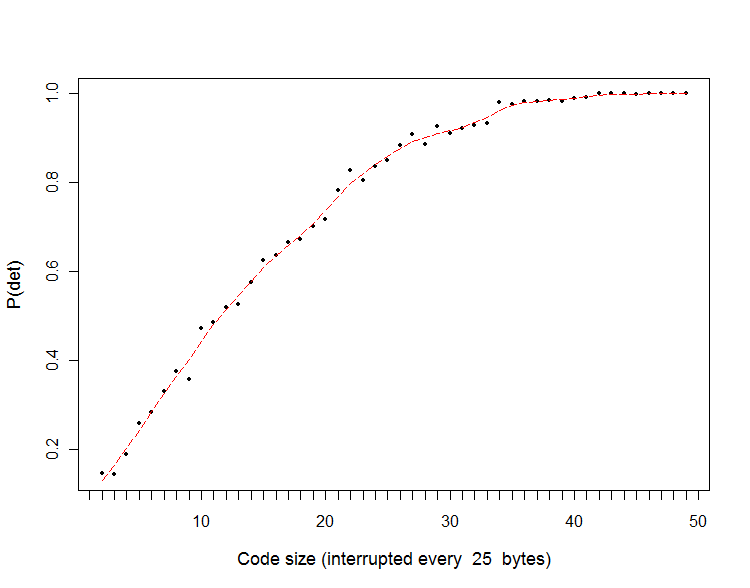
\includegraphics[scale=0.5]{images/bubble_det_codesize}
\caption{{Probability of detection versus size of injected code.}}
\vspace{0.3cm}
\label{det_codesize}
\end{center}
\end{figure}


In the numerical simulation which confirms this probability, sprayed memory is interrupted according to the parameters of the countermeasure described above. For each variation of parameters such as size of injected code and interruption rate, the simulation has been run several times and the final number of detections is obtained by averaging across 1000 experiments. We believe this strategy to be capable of returning robust results.

In Figure \ref{det_codesize} we show a graph of the probability of detection versus the size of the injected code, at the highest level of security. When the injected code is smaller than $10$ bytes the probability of interrupting it and detecting the attack upon code execution, is less than $40\%$.
Fortunately, this probability increases very quickly for codes of larger sizes and goes practically to $100\%$ (certain detection) when the attacker injects a code larger than $42$ bytes.  

Another variable that not only determines the level of security but also the overall performance impact of the countermeasure is the interruption rate. In order to achieve better performance this variable can be set to higher values, at the cost of decreasing the level of security. In Figure \ref{det_intrate} we show the probability of detection for injected code of several sizes versus the interruption rate. We are confident this to represent a better picture that should be considered before tuning the interruption rate in order to have a countermeasure with a smaller performance impact.


\begin{figure}[htbp] 
\begin{center}
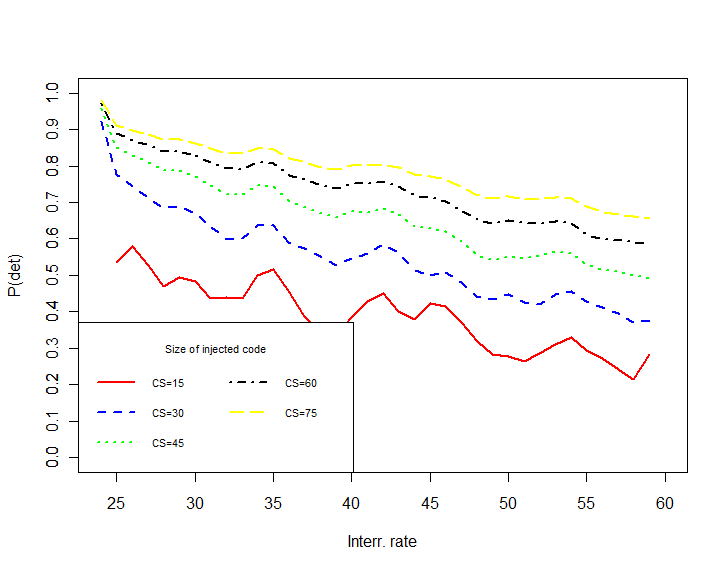
\includegraphics[scale=0.5]{images/bubble_det_intrate}
\caption{{Probability of detection compared to detection rates for injected code of several sizes}}
\vspace{0.3cm}
\label{det_intrate}
\end{center}
\end{figure}



An interesting scenario would arise if an attacker breaks the 25-byte shellcode in smaller chunks, not only to fit in the limited interrupted space but also to decrease the probability of detection. Therefore, he concatenates each chunk by using \emph{JMP relx} instructions\footnote{On the Intel architecture \emph{JMP relx} indicates an instruction that sets the Instruction Pointer to a relative offset of 8,16 or 32 bits.}. 
Clearly, each chunk can be stored in the memory space interrupted every $25$ bytes and, according to the aforementioned simulation, the probability of successful execution of that code would be $1 - P(detection) = 1 - 0.4 = 0.6$. 
Assuming the attacker is concatenating chunks of 10 bytes using \emph{JMP rel8} instructions (2 bytes on the Intel architecture), there will be space for only $10-2 = 8$ bytes of shellcode per chunk. Therefore, the number of chunks needed to form the complete 25 byte shellcode amounts to $\lceil \frac{25}{8} \rceil = 4$. 
The assumption of independency between chunks and special interruption bytes provides an estimate of the probability of executing 4 adjacent chunks equal to $0.6^4 = 0.13$.  This represents the best case scenario for the attacker who has complete knowledge of the memory layout and can jump directly to the beginning of his shellcode without the aid of NOP sleds. In realistic conditions this knowledge is not present.

As already mentioned, the reliability of heap-spraying attacks is due to the usage of code sleds that drive the Instruction Pointer from inaccurate memory locations to the shellcode. The use of NOP sleds dramatically increases the size of injected code. Therefore, although we consider these attacks feasible from a probabilistic point of view, they are quite hard to be realised in practice with reasonable reliability.



\section{Hypervisor integration}\label{bub:integration}
Despite the numerous possibilities that virtualisation technology can offer to the end user, we will focus on a specific case of virtualised desktop. The environment we refer to in this section is the one used to deliver web browsers on demand. 

A virtual machine for each web browser is deployed in order to guarantee mobility, consistency of view and security. Mobility allows the user to access his own private desktop from anywhere, using any device and maintaining a consistent look and feel among them. It should be clear that, in such an environment, security by isolation is achieved by design. In fact, all the virtual machines are running on top of a hypervisor executing on virtualisation-enabled hardware.

However, considering an application more secure and shielded just because it is running within a virtual machine is a type of misunderstanding that is becoming more and more common, specially in the industry \cite{virtoverkill}. Specifically to the environment we described, isolating virtual machines would not prevent attacks to the single web browser. Executing an instance of the web browser within a virtual machine does not make it immune to common attacks. Therefore, if that web browser loads a malicious page where a heap-spraying attack has been implemented, the chances of successful attack are equivalent to those of a browser running within a physical machine. 

However, if a countermeasure like the one described before is in place, precious information about the attack can be collected and used to reduce the risk of attacks to the rest of the infrastructure. The other virtual machines running on top of the same hypervisor can be informed of the malicious address that caused the attack. 

As mentioned before, executing the $0xCC$ byte should be a convincing evidence of an on-going heap-based attack on the browser's heap. Moreover, when the operating system has been virtualised, the $0xCC$ interrupt handler implemented in the guest kernel can interact with the hypervisor in a straightforward way, via the raise of a hypercall as described in Chapter \ref{virt:paradigm}. This mechanism is used not only to notify  an attempt of execution of malicious code to the hypervisor, but also to update a blacklist of URLs that caused such an attack.
A schema of such an environment is provided in Figure \ref{virtualdesktop}.

\begin{figure}[t!]
\begin{center}
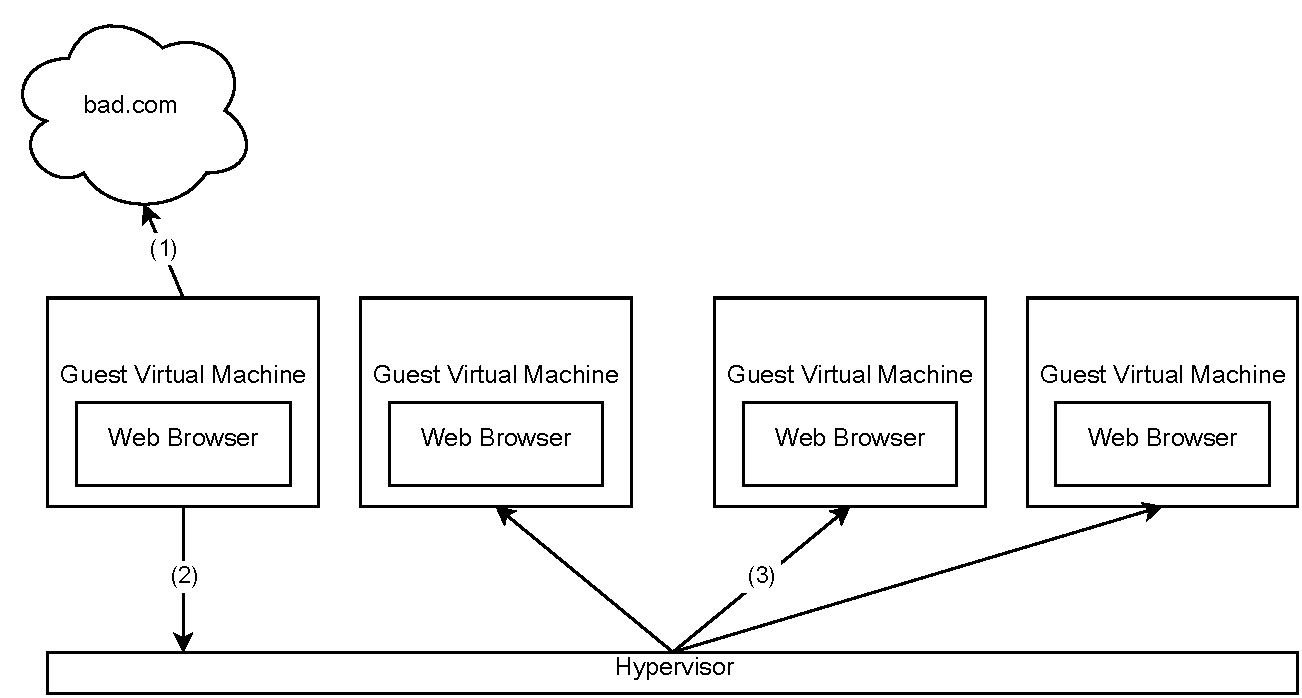
\includegraphics[scale=0.55]{images/virtualDesktop.pdf}
\caption{{Schema of hypervisor integration: upon loading malicious content from bad.com (1) and local detection of  heap-based attack, the guest notifies the hypervisor (2) sending the malicious URL that caused the attack. The hypervisor will deliver this information to all virtual machines running on top (3) or, alternatively will update a blacklist in its private space.}}
\vspace{0.3cm}
\label{virtualdesktop}
\end{center}
\end{figure}


Once a heap-spraying attack has been detected, two main strategies might be considered:  

\begin{itemize}
\item deliver the blacklist of malicious URLs to the virtual machines that will, in turn, update their network filters and prevent the local web browsers from navigating to these addresses or 

\item keep the aforementioned blacklist in the hypervisor's space. 
\end{itemize}

Since the hypervisor has access to physical network devices and it opens network connections on behalf of the virtual machines running on top, we believe that the second choice is to be preferred. 
A centralised blacklist results easier to keep up to date. Moreover, the isolation mechanism will even protect this information from any attempt of compromising or deleting it from the guest kernel.
 
Clearly, in those cases in which virtual machines need to be migrated to other hypervisors, for the reasons that are out of the scope of this work, decentralising the blacklist and delivering it to the single guest machines will be essential to keep the guests protected even after their migration has occurred.

Regardless the choice of strategy, further access to malicious network address will be denied to browsers running within the virtualised environment.



%Another scenario that shows the great advantage of integrating local countermeasures with hypervisor technology is  session migration to pristine environments. 
%
%Due to the assumption that a strict security measure should not consider a kernel trustworthy after a heap-based attack has occurred, we believe that security critical applications for which continuity must be granted, should be executed on non compromised kernels without being interrupted. 
%Therefore, we address the needs to migrate such applications to a machine and operating system that are known to be in an clean state.
%A solution to such an issue is offered by our in-guest countermeasure described in Chapter \ref{hyperforce}, working in cooperation with the hypervisor.

%\begin{figure}[t]
%\begin{center}
%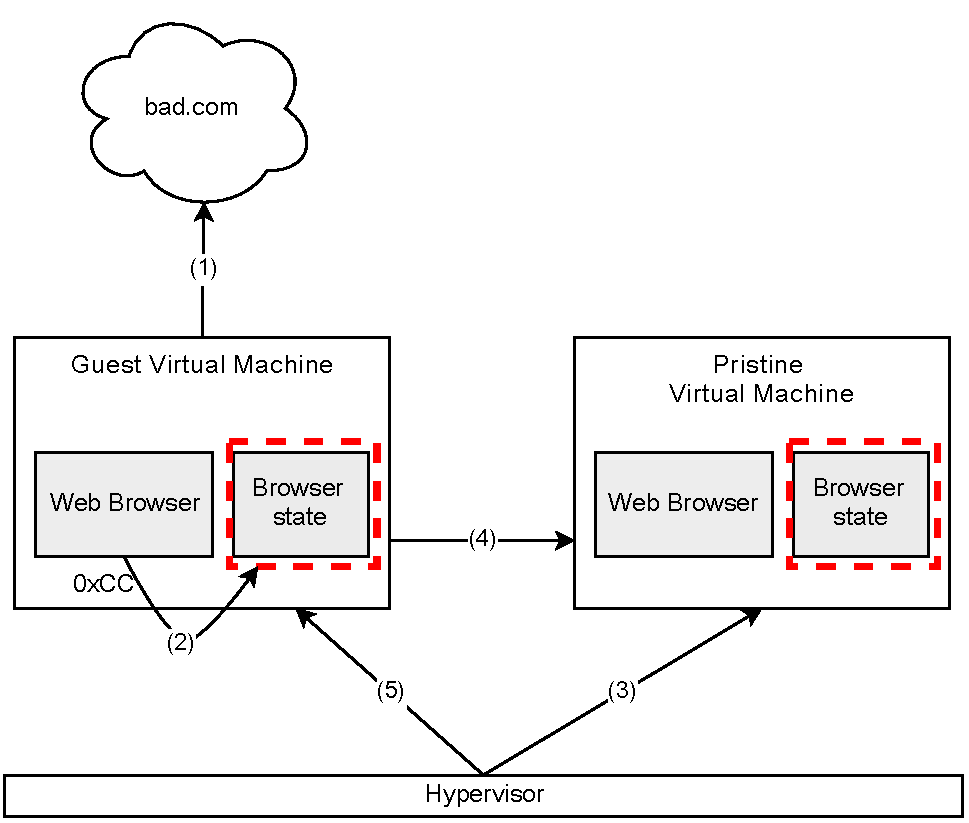
\includegraphics[scale=0.6]{images/pristine.pdf}
%\caption{{Session migration into a pristine virtual machine. A heap-based attack is triggered by visiting a malicious web page (1). Upon notification of the attack (2) the hypervisor starts a new virtual machine (3), migrates the browser state from the old virtual machine to the new one (4) and destroys the potentially compromised guest (5)}}
%\label{pristine}
%\end{center}
%\end{figure}


%The migration strategy includes 1) starting a new guest machine to which opening connections to the blacklisted URL that caused the attack is denied 2) save the browser state from the old machine and 3) restoring the browser state within a new instance of a web browser running within a clean kernel.
%
%A schema of the session migration strategy we propose is provided in Figure \ref{pristine}. 


%In order to implement one of the security measures that have been addressed above, the enforcing framework described in Chapter \ref{hyperforce} can be taken into consideration. By adding the special byte $0xCC$ as a non-maskable interrupt, secure code execution will be enforced as a regular interrupt handler. This code, which is stored in a memory area protected by the hypervisor, will take a snapshot of the browser running state together with values of document objects, values entered in forms by the user, browser history and cookies. Code executing natively within the guest will facilitate the access to the browser data structures by reducing the semantic gap between the virtual machine and the hypervisor. Moreover, as shown in Chapter \ref{hyperforce} will execute faster than the equivalent code running outside the virtual machine. 
%Once the hypervisor has started a new disposable virtual machine, the browser state has been copied to the protected memory area of the new machine and a new instance of the web browser has been launched, the old browser state can be restored and its execution resumed. Finally the old virtual machine, running a potentially compromised kernel, will be deleted in order to free resources.
%We argue that browser session migration strategies like the one described in \cite{browsermigration} can be easily integrated within the Hyperforce framework. 


\section{Related work}\label{bub:related}
In this section we provide some of the most effective countermeasures related to web browser security developed so far. Several countermeasures, like the ones described in Section \ref{cmnozzle}, have been designed and implemented to specifically protect against heap-spraying attacks. Others have been designed to prevent memory corruption in general, like those in Section \ref{sul}. 
Two architectures that take advantage of virtualisation technology to provide coarse grained isolation of user applications are described in Section \ref{virtbased}. 
%We provide an overview of some countermeasures against heap overflow attacks in Section \ref{sul}. A description of some countermeasures specifically designed to protect against heap-spraying attacks in web browsers is provided in Section \ref{cmnozzle}. 

\subsection{Heap-spraying defences} \label{cmnozzle}

\paragraph{Nozzle} 
Nozzle is the first countermeasure specifically designed against heap-spraying attacks via web browsers \cite{nozzle08tr}. It uses emulation techniques to detect the presence of malicious objects. This is achieved by the analysis of the contents of any object allocated by the web browser. The countermeasure is in fact implemented at the memory allocator level. This has the benefit of protecting against a heap-spraying attack by any scripting language supported by the browser.
Each block on the heap is disassembled and a control flow graph of the decoded instructions is built. A \texttt{NOP-shellcode} object may be easily detected because one basic block in the control flow graph will be reachable by several directions (other basic blocks). For each object on the heap a measure of the likelihood of landing within the same object is computed. This measure is called \texttt{attack surface area}. The surface area for the entire heap is given by the accumulation of the surface area of individual blocks. This metric reflects the overall heap \textit{health}. 
This countermeasure is more compatible than DEP and would help to detect and report heap-spraying attacks by handling exceptions, without just crashing. This approach has although some limitations. Because Nozzle examines objects only at specific times, this may lead to the so called TOCTOU-vulnerability (Time-Of-Check-Time-Of-Use). This means that an attacker can allocate a benign object, wait for Nozzle to examine it, then change it to contain malicious content and trigger the attack. Moreover, Nozzle examines only a subset of the heap, due to performance reasons. But this approach will lead to a lower level of security. The performance overhead of Nozzle examining the whole heap is unacceptable for every day computing.
Another limitation of Nozzle comes from the assumption that a heap-spraying attack allocates a relatively small number of large objects. A design based on this assumption would not protect against another type of heap-spraying attack which allocates a large number of small objects instead, which is known to have the same probability to succeed. 
%OK


\paragraph{Shellcode detection}
Another countermeasure specifically designed against heap-spraying attacks to web browsers is proposed by \cite{EURECOM}. This countermeasure is based on the assumptions that (1) a heap-spraying attack may be conducted by a special crafted HTML page instrumented with Javascript and (2) Javascript strings are the only way to allocate contiguous data on the heap. Thus all strings allocated by the Javascript interpreter are monitored and checked for the presence of shellcode. All checks have to be performed before a vulnerability can be abused to change the execution control flow of the application. If the system detects the presence of shellcode, the execution of the script is stopped. Shellcode detection is performed by \emph{libemu}, a small library written in C that offers basic x86 emulation. Since \emph{libemu} uses a number of heuristics to discriminate random instructions from actual shellcode, false positives may still occur. Moreover an optimised version of the countermeasure that achieves accurate detection with no false positives is affected by a significant performance penalty of 170\%.
%OK
 
\subsection{Alternative countermeasures} \label{sul}

\paragraph{Probabilistic countermeasures}
Many countermeasures make use of randomness when protecting against attacks. Canary-based countermeasures \cite{Krennmair:2003:CLE,Robertson:2003:RTD} 
%%Cowan:1998:SAA,Etoh:2000:PSS
use a secret random number that is stored before an important memory location: if the random number has changed after some operations have been performed, then an attack has been detected. Memory-obfuscation countermeasures \cite{Bhatkar:2008:DSR,Cowan:2003:PPP} encrypt (usually with XOR) important memory locations or other information using random numbers.  The memory layout is usually randomised as in \cite{Bhatkar:2003:AOE,Bhatkar:2005:ETC,Xu:2003:TRR}, 
%%Team:20xx:DPP,
by loading the stack and heap at random addresses and by placing random gaps between objects. 
Another type of randomisation consists in encrypting the entire instruction set of an architecture \cite{Barrantes:2003:RIS}
before fetching the instructions and decrypting them before they are executed. While these approaches are often efficient, they rely on keeping memory locations secret. Unfortunately, programs that contain buffer overflows could also be affected by  \emph{buffer overreads} vulnerabilities (e.g. a string which is copied via \emph{strncpy} but not explicitly null-terminated could leak information) or format string vulnerabilities, which allow attackers to print out memory locations. Such memory leaking vulnerabilities could allow attackers to bypass this type of countermeasure. Another drawback of these countermeasures is that, while they can be effective against remote attackers, they can be easily bypassed locally, via brute force attacks on the secret areas.
 
\paragraph{DEP}
Data Execution Prevention \cite{dep} is a countermeasure designed to prevent the execution of code in memory pages. It is implemented  either in software or hardware, via the NX bit. With DEP enabled, pages will be marked non-executable and this will prevent the attacker from executing shellcode injected on the stack or the heap of the application. If an application attempts to execute code from a page marked by DEP, an access violation exception will be raised. This will lead to a crash, if not properly handled. While the aforementioned hardware-based countermeasure is recognised as effective against code injection attacks, its main limitation consists in the fact that several applications attempt to execute code from memory pages. 
Due to these types of compatibility issues, the deployment of DEP is less straightforward than it should be \cite{depdef}.

\paragraph{Separation and replication of information}
Countermeasures that rely on separation or replication of information will try to replicate valuable control-flow information \cite{Younan:2006:EPA,Younan:2006:EPA2, Chiueh:2001:RCT, Vendicator:20xx:DS} or will separate this information from regular data. This makes it harder for an attacker to overwrite these critical memory areas using an overflow. Some countermeasures will simply copy the return address from the stack to a separate stack and will compare it to or replace the return addresses on the regular stack before returning from a function. These countermeasures are easily bypassed using indirect pointer overwriting by which an attacker overwrites a different memory location instead of the return address exploiting a pointer from the stack. More advanced techniques try to separate all control-flow data (like return addresses and pointers) from regular data, making it harder for an attacker to use an overflow to overwrite this type of data.
While these techniques can efficiently protect against buffer overflows that try to overwrite control-flow information, they do not protect against attacks where an attacker controls an integer that is used as an offset from a pointer, nor do they protect against non-control-data attacks.
%OK


%\paragraph{Execution monitors}
%The countermeasures described below are capable of monitoring the execution of a program and preventing the transfer of control-flow which could be unsafe. 
%
%Program shepherding \cite{Kiriansky:2002:SEP} is a technique that monitors the execution of a program and will disallow control-flow transfers that are not considered safe. Such a control flow transfer occurs when e.g., a \emph{call} or \emph{ret} instruction is executed. 
%An example of a use for shepherding is to enforce return instructions to only return to the instruction after the call site. The proposed implementation of this countermeasure is done using a runtime binary interpreter. As a result, the performance impact of this countermeasure is significant for some programs, but acceptable for others.
%Control-flow integrity \cite{Abadi:2005:CFI} determines a program's control flow graph beforehand and ensures that the program adheres to it. It does this by assigning  a unique ID to each possible control flow destination of a control flow transfer. Before transferring control flow to such a destination, the ID of the destination is compared to the expected ID, and if they are equal, the program proceeds as normal.  This approach, while strong and in the same efficiency range as our approach, does not protect against non-control data attacks.

\paragraph{Virtual Browser}
A work that borrows the concepts of virtualisation technology and applies them to the development of secure web browsers is provided in \cite{virtualbrowser}. Virtual Browser is a browser-level virtualised environment that executes third party Javascript code in isolation from the rest of the system, namely other components of the web browser itself and the host system. The isolated components can still communicate with each other through data flows that have been carefully examined with security in mind. 
The idea of Virtual Browser is very similar to that of virtual machines. It provides its own HTML and CSS parsers and a Javascript interpreter. Therefore, untrusted Javascript code is parsed and executed within the isolated environment, preventing the exploitation of bugs in the main Javascript interpreter of the browser.
For the same reason, trusted Javascript can execute within the native Javascript engine, improving the overall performance of the countermeasure. The performance overhead is comparable to the Microsoft Web Sandbox, but the degree of security is higher and a more complete Javascript language is supported.
An important feature that makes Virtual Browser readily deployable is that it is written in a language that is supported by the native browser (a Javascript implementation is provided). Therefore, no modification to the browser codebase is required. Virtual Browser provides isolation of the Javascript interpreter, leaving all other means to attack web browsers unprotected. Although a direct comparison with Web Sandbox shows that Virtual Browser outperforms it in some cases, the overhead compared to web browsers running natively is not negligible. 
%OK


\subsection{Virtualisation-based countermeasures}\label{virtbased}
\paragraph{QubesOS}
The development of a virtualisation-based Linux distribution like QubesOS \cite{qubesos} has been driven by the inability of traditional operating systems to provide isolation among different applications running within the same machine.  This is the main reason for which current operating systems are usually not capable of protecting other user's applications and data from being compromised when an application, for instance the web browser, has been attacked by a malicious website. 
This concept has been extended to the other components of the operating system. Exploiting a bug in the network stack can affect the security of other applications and their data, without the operating system to notice and defend potential targets.
Virtualisation is the chief technology QubesOS is based on, due to its security isolation properties. The main idea of QubesOS is to execute a number of guests, also called \emph{disposable virtual machines}, in which applications that need to stay isolated during their lifetime are executed. The entire system is based on disposable virtual machines such as the social virtual machine, in which applications like the email client or any other web social service will be executed, the shopping virtual machine, used for those applications to purchase goods from the Internet with a credit card, or the corporate virtual machine, where the corporate email client or VPN connections will take place. 
If one of the aforementioned virtual machines gets compromised, applications and data running in the other ones will stay isolated and their code untampered.
Disposable virtual machines are not only used for regular applications but also for system services such as the network system, the graphical or the storage subsystems. A bug in one of those subsystems will stay isolated for the same reasons explained above.
QubesOS is a hybrid architecture that takes the concept of isolation, typical of microkernel systems, in which device drivers are not part of the core kernel and run in unprivileged mode, and the flexibility of monolithic systems.
The challenging task of QubesOS consists in allowing virtual machines to share data among each other and still maintain the overall system safe. For instance, those applications that are being run in different virtual machines might need their data to be shared; the web browser isolated in the social virtual machine will certainly use the network system, provided by the network virtual machine in which the NIC driver, the TCP/IP stack and 802.11 stack are running; most of the applications running in their own virtual machines will need the graphical subsystem for basic human-computer interaction, provided by the GUI virtual machine. 
All the required inter-connectivity is provided by the Xen hypervisor that takes advantage of hardware supported virtualisation technology. Despite the high demand in terms of hardware resources and the performance impact that depends on the number of virtual machines running simultaneously, QubesOS is one of the few systems that can guarantee strong isolation at application level.

\paragraph{Invincea}
A commercial product originally designed to isolate web browsers in virtual execution environments within a virtualisation platform is presented in \cite{invincea}.
Due to the proprietary nature of Invincea software, no details about its technical implementation are provided.
However, the main goal of the product is to protect the host operating system from malware that targets mainly the web browser as a spreading medium. Whenever the browser protection detects a malware threat, the user is informed and the virtual environment in which the browser is executing is shut down. At this point a new disposable virtual machine is started in order to minimise user interruption. Hardware-supported virtualisation is used to provide the required separation.
The main feature of Invincea consists in the fact that it relies on unusual behaviour of an application in the virtual environment rather than on malware signature. Moreover, the data collected during a malware attack is sent to centralised data servers to be analysed and to build a collective intelligence database that may protect other clients.
This type of protection has been extended to PDF file readers, office suite, compressed and executable files, in a more recent release of the product. 


\section{Summary} \label{bub:conclusion}
%%Other programs in user space can benefit from virtualisation support with a similar mechanism (adobe reader, flash, interpreted language engines) 
A recent heap-based attack to web browsers revealed to be effective and capable of circumventing countermeasures that have been specifically designed against these types of threats. 
Heap-spraying attacks expect to have large parts of the heap to be homogeneous, a requirement that is fulfilled a number of times in a complex application like the web browser. 
In this chapter we show that, by introducing heterogeneity where attackers expect this homogeneity, we can make heap-based buffer overflows a lot harder. 

We provide a proof-of-concept, by modifying the Javascript engine internal representation of the string data type of a widely used web browser. We show how effective is introducing diversity against such attacks. This is done by inserting special values at random locations in the string, which will cause a breakpoint exception to occur if they are executed. 
%If an attacker tries to perform a heap-spraying attack, his injected code will now have been interrupted at a random location with such a breakpoint exception, allowing the browser to detect and report that an attack has occurred. 
Benchmarks show that this countermeasure has very limited impact, both in terms of performance at runtime and memory overhead.

In addition to the single-browser scenario we explain the case in which the target application is running in a virtualised operating system. We show how this countermeasure can be easily integrated with the virtualisation infrastructure and take advantage of hypervisor capabilities to protect other peers in a \emph{attack-once-protect-everywhere} fashion. 

%Moreover, for those environments with high security requirements and the need for business continuity, our approach can be considered to migrate sessions (in the case of a web browser) to a pristine operating system, upon notification of attack.

Although we implemented a prototype for a widely adopted web browser, the concepts described in this chapter hold to many other scenarios like those in which interpreted language engines are embedded in user space applications and that are vulnerable to the same type of attack. 
